\section{Introduction}
Temporal Networks scheduling algorithms support diverse formulations useful in modeling practical problems. Examples include dynamical execution strategies based on partial knowledge of uncertain durations, or strategies upper-bound the probability of failing to satisfy probabilistic constraints. However, it is not obvious how to apply them in scenarios with resource usage constraints. Those kind of scenarios, on the other hand are investigated in Operations Research literature and known as project scheduling. Time Resource Network attempt to narrow the gap between those two bodies of work, which so far remained mostly independent.

Let's consider the following Smart House scenario. We have $150W$ generator which is available. We know that the user comes back from work at some time defined by a gaussian distribution $N(5pm, 5m)$. Moreover we know that sun sets at time defined by $N(7pm, 1m)$. We would like to meet the following constraints with the overall probability at least $98\%$:
\begin{itemize}
\item Wash clothes (duration: $2h$, power usage: $130W$) before user comes back from work
\item Cook dinner (duration: $30m$, power usage: $100W$) ready within 15 minutes of user coming back from work
\item Have the lights on (power usage: $80W$) from before sunset to at least midnight.
\item Cook a late night snack (duration: $30m$, power usage: $20W$) between 10pm and 11pm.
\end{itemize}
While probabilistic constraints can be straightforwardly modeled using probabilistic Simple Temporal Networks \cite{Fang2014}, there is no known algorithm that can jointly model the resource constraint. In this publication we introduce Time Resource Networks, which are capable of finding schedules for this type of scenarios. Solution to the example described above is presented on fig. \ref{fig:pstnu_scheduling}. In meets the constraints with $99,7\%$ probability.


\begin{figure}[H]
\begin{center}
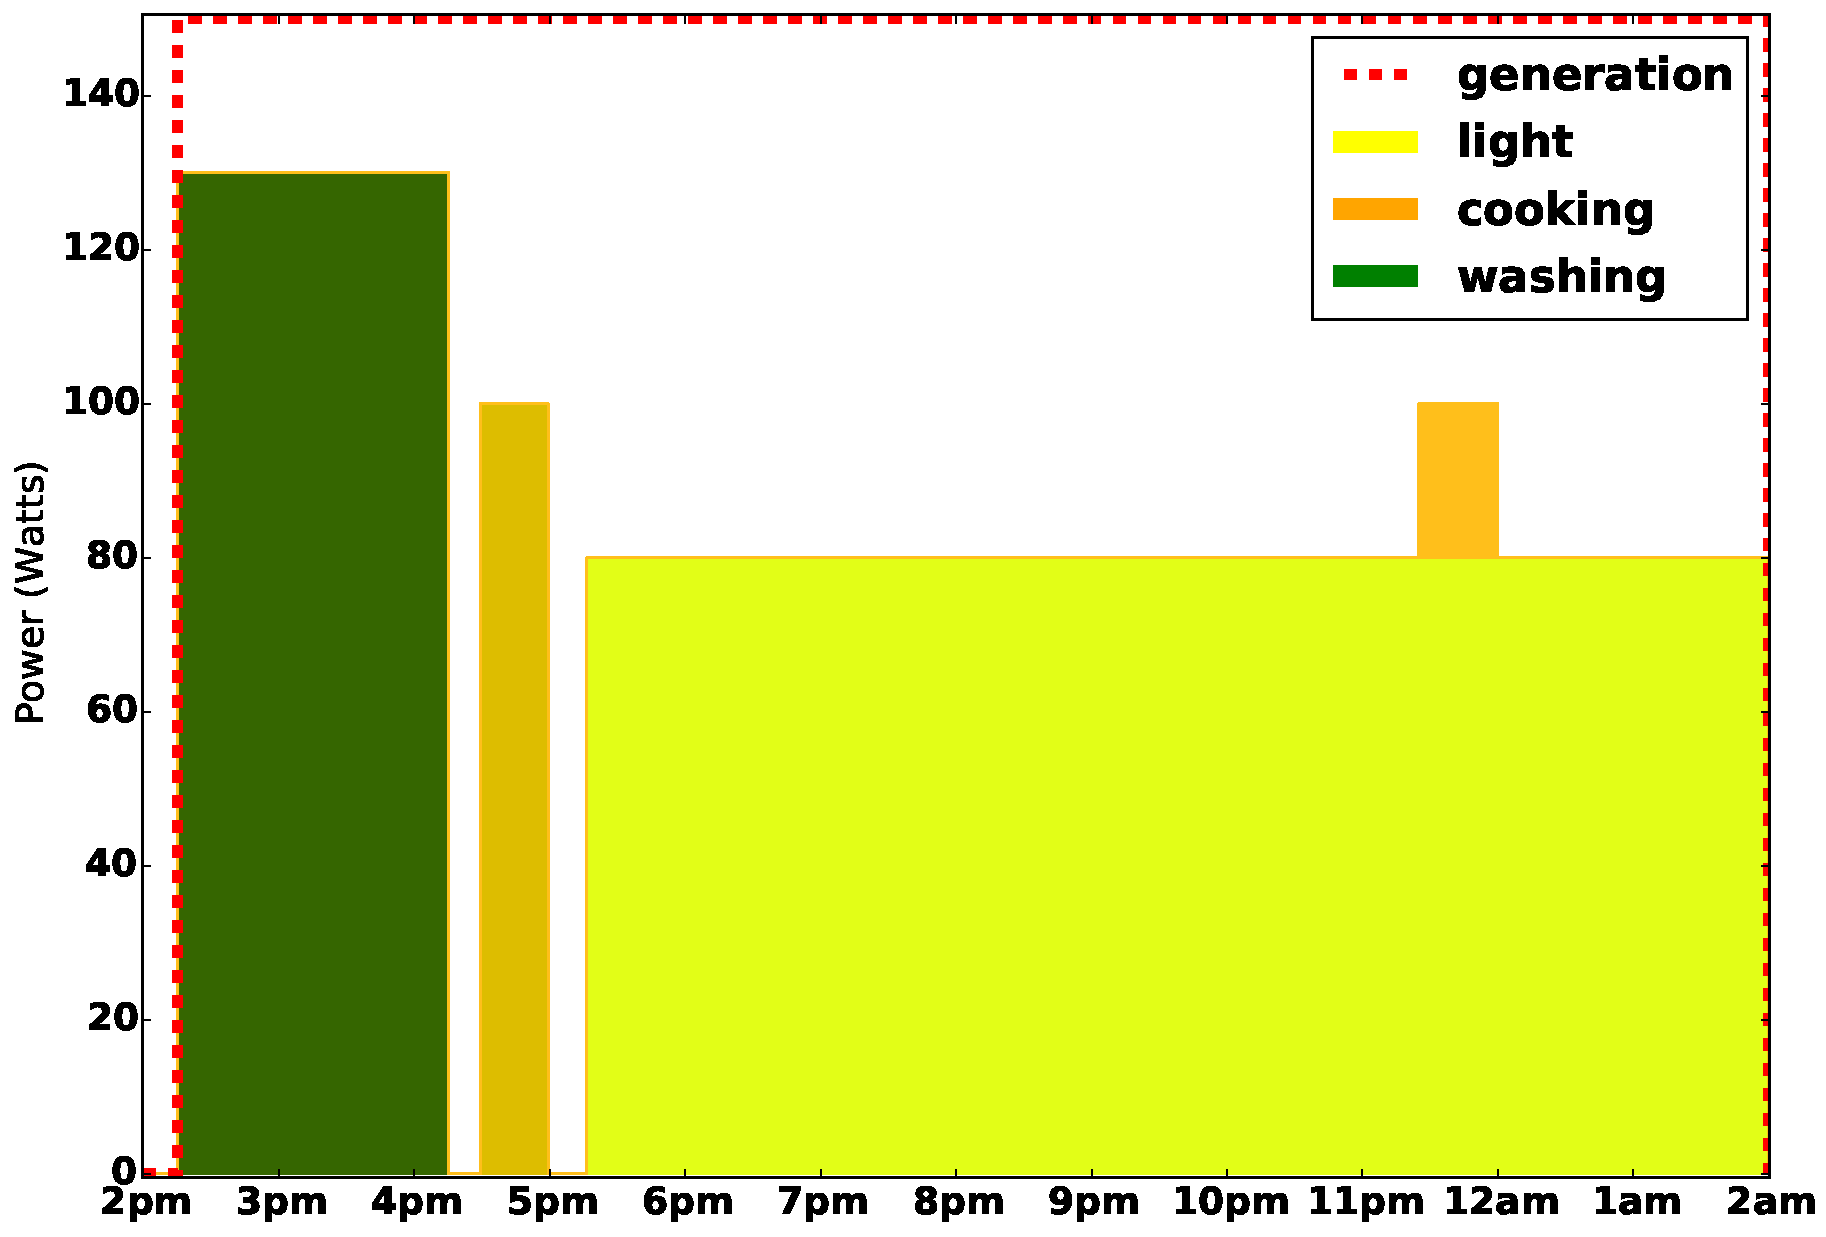
\includegraphics[width=0.49\textwidth]{pstnu_scheduling}
\caption{Depiction of solution to TRN spanning a pSTN.}
\label{fig:pstnu_scheduling}
\end{center}
\end{figure}
